\documentclass[times,10pt,twocolumn]{article}
\usepackage[latin1]{inputenc}
\usepackage{latex8}
\usepackage{times}
\usepackage{comment}
\usepackage{epsfig}
\usepackage{amssymb}
\usepackage{float}
\usepackage{boxedminipage}
\usepackage{algorithm}
\usepackage{url}
\urlstyle{sf}
\usepackage{fullpage}
\usepackage{alltt}
\usepackage[usenames]{color}
\usepackage{graphics}




%%% ENVIRONMENTS
\newtheorem{theorem}{Theorem}
\newtheorem{prop}[theorem]{Proposition}
\newtheorem{lemma}[theorem]{Lemma}
\newtheorem{definition}[theorem]{Definition}
\newtheorem{example}{Example}
\newtheorem{remark}{Remark}

%%%


\newcommand{\ie}{\emph{i.e.}}
\newcommand{\eg}{\emph{e.g.}}
\newcommand{\verbi}[1]{{\small\texttt{#1}}}


%% Intra nos
\newcommand{\Ce} [1]{{[\color{cyan}{C�dric}}: {#1}]}
\newcommand{\Fr} [1]{{[\color{blue}{Francesco}} {#1}]}
\newcommand{\Lu} [1]{{[\color{red}{Luigi}}: {#1}]}
\newcommand{\RESP} [1]{{[\color{red}{RESP: #1}]}}


%%%% FORMATTING
\newcommand{\rew}[1]   {\hspace{-#1mm}}
\newcommand{\fwd}[1]   {\hspace{#1mm}}
\newcommand{\down}[1]  {\vspace{#1mm}}
\newcommand{\up}[1]    {\vspace{-#1mm}}



\usepackage{algorithm}

\newfloat{algo}{thp}{}
\floatname{algo}{Algorithm}

\newcommand{\R}{\mathtt{root}}

\newcommand{\TRUE}{\mathtt{true}}
\newcommand{\FALSE}{\mathtt{false}}
%\newcommand{\R}{\mathtt{R}}
%\newcommand{\C}{\mathcal{C}}
%\newcommand{\OR}{\mathtt{O}}
\newcommand{\IF}[1]{\textbf{if} {#1}}
\newcommand{\THEN}{\textbf{then} }
\newcommand{\ELSE}{\textbf{else} }
\newcommand{\ELSEIF}[1]{\textbf{elseif} {#1}}
\newcommand{\ENDIF}{\textbf{endif} }
\newcommand{\FOR}[1]{\textbf{for} {#1} \textbf{do }}
%\newcommand{\FOR}[2]{\textbf{for } {#1} \textbf{to } {#2} \textbf{do }}
\newcommand{\FORALL}[1]{\textbf{for all} {#1} \textbf{do }}
\newcommand{\FOREACH}[1]{\textbf{for each} {#1} \textbf{do }}
\newcommand{\WHILE}[1]{\textbf{while} {#1} \textbf{do }}
\newcommand{\REPEAT}{\textbf{repeat} }
\newcommand{\FOREVER}{\textbf{forever} }
\newcommand{\DONE}{ \textbf{done}}

\newcommand{\ALGOHEADER}[3]
{\begin{tabular}[t]{@{\extracolsep{0pt}}p{#3}l}
    \textbf{#1} &
    \begin{tabular}[t]{@{\hspace{15pt}}l}
        #2
    \end{tabular}
 \end{tabular}\smallskip
}

\makeatletter
\newcommand{\alglabel}[1]{%
  \@bsphack%
  \protected@write\@auxout{}%
         {\string\newlabel{#1}{{\the\ALGONum\LineSep \formatLine}{\thepage}}}
  \@esphack%
}
\makeatother

\newcommand{\CST}[1]      {\ALGOHEADER{Constants: }{#1}{.5in}}
\newcommand{\VAR}[1]        {\ALGOHEADER{Variables: }{#1}{.5in}}
\newcommand{\LOCALVAR}[1]   {\ALGOHEADER{Local  Variables: }{#1}{1.2in}}

\newcommand{\MACRO}[1]      {\ALGOHEADER{Macros: }{#1}{.5in}}

%\newcommand{\FUNCTION}[2]   {\textbf{function}  ${#1}$: \textbf{{#2}}}

\newcommand{\FUNCTION}[1]{\textbf{Function} {#1}}

\newcommand{\RETURN}[1]     {\textbf{return} {#1}}
\newcommand{\PROC}[1]       {\textbf{procedure} ${#1}$}
\newcommand{\INIT}[1]       {\textbf{initially} ${#1}$}
\newcommand{\ACTION}        {\textbf{actions:}}

\newcommand{\MAC}[2]
{
   ${#1} \equiv $
   \begin{tabular}[t]{@{\extracolsep{0pt}}l}
       #2
   \end{tabular}
}

\newcommand{\RCV}[1]{\textbf{upon} receipt \textbf{of} $<$#1$>$ \textbf{do}}
\newcommand{\RCVFROM}[2]{\textbf{upon} receipt \textbf{of} $<$#1$>$ \textbf{from} #2 \textbf{do}}
\newcommand{\RCVFROMSYNC}[2]{\textbf{receive} $<$#1$>$ \textbf{from} #2} %\textbf{to} #2}

\newcommand{\SEND}[2]{\textbf{send} $<$#1$>$ \textbf{to} #2}
\newcommand{\SENDSYNC}[2]{\textbf{send-sync} $<$#1$>$ \textbf{to} #2}
\newcommand{\SENDTOHOST}[1]{\textbf{send\_to\_host}$<$#1$>$}
\newcommand{\RCVFROMHOST}[1]{\textbf{receive\_from\_host}$<$#1$>$}

\newcommand{\PROCINIT}{\textbf{upon} INITIALIZATION}

\newcommand{\BEGLIST}{\begin{list}{}{\partopsep -3pt \parsep -2pt \listparindent -0pt \labelwidth .5in}}
\newcommand{\ENDLIST}{\end{list}}
\newcount\ALGOLine
\ALGOLine=-1
\newcount\ALGOLineStart
\ALGOLine=0
\newcount\ALGONum
\ALGONum=1

\newcommand{\LineSep}{.}
\newcommand{\LINESTYLE}{\scriptsize}
\newcommand{\INITALGO}[1]{\global\ALGONum=#1}
\newcommand{\INITLINE}[1]{\global\ALGOLineStart=#1}
\newcommand{\RESETLINE}{\global\ALGOLine=\ALGOLineStart}
\newcommand{\formatLine}{\ifnum\the\ALGOLine<10 0\fi\the\ALGOLine}
\newcommand{\NA}{\global\advance\ALGONum  by 1 \RESETLINE}
\newcommand{\AL}{\global\advance\ALGOLine by 1 \LINESTYLE{$\the\ALGONum$\LineSep$\formatLine$}}
\newcommand{\VL}{\ \vline\>}

\newcommand{\logreq}{{\tt logReq}}
\newcommand{\hostreq}{{\tt hostReq}}
\newcommand{\updatechild}{{\tt updateChild}}
\newcommand{\addchild}{{\tt addChild}}
\newcommand{\scanreq}{{\tt scanReq}}
\newcommand{\replicationreq}{{\tt replicationReq}}
\newcommand{\addparent}{{\tt addParent}}

\newcommand{\commonprefix}{{\bf COMMONPREFIX}}
\newcommand{\sizeof}{{\bf SIZEOF}}
\newcommand{\getpeer}{{\bf GETPEER}}
\newcommand{\getnbreplicas}{{\bf GETNBREPLICAS}}
\newcommand{\getbestreplica}{{\bf GETBESTREPLICA}}

\newcommand{\PREF}[1]{\mbox{{\sc Prefixes}}({#1})}

%%%%% ASYNC REPAIR
\newcommand{\destroy}{{\footnotesize{\bf DESTROY}}}
\newcommand{\prefix}{{\footnotesize{\bf PREFIX}}}
\newcommand{\isprefix}{\sc IsPrefix}
\newcommand{\len}{{\footnotesize{\bf LEN}}}
\newcommand{\gcp}{{\footnotesize{\bf GCP}}}
\newcommand{\inser}{{\footnotesize{\bf INSERT}}}
\newcommand{\newnode}{\sc NewNode}

\newcommand{\checkmerge}{\sc CheckMerge}
\newcommand{\checkdown}{\sc CheckDown}
\newcommand{\checkup}{\sc CheckUp}
\newcommand{\checkdef}{\sc CheckDefault}

\newcommand{\msgmerge}{\sc MsgMerge}
\newcommand{\msgdown}{\sc MsgDown}
\newcommand{\msgup}{\sc MsgUp}
\newcommand{\msgdef}{\sc MsgDefault}

\newcommand{\Bt}{B\mbox{-}tree}

%\newtheorem{theorem}{Theorem}
%% \newtheorem{hypothese}{Hypothèse}
%% \newtheorem{lemma}{Lemma}
%% \newtheorem{corollary}{Corollary}
%% \newtheorem{proposition}{Proposition}
%% \newtheorem{definition}{Definition}
%% \newtheorem{assumption}{Assumption}
%\newtheorem{remark}{Remark}

\floatname{algorithm}{Algorithm}

\newcommand{\phyreq}{{\tt phyReq}}
\newcommand{\phyreqinitiator}{{\tt phyReqInitiator}}
\newcommand{\updatesuccessor}{{\tt updateSuccessor}}
\newcommand{\host}{{\bf INSERT}}

\floatname{algorithm}{Algorithm}

\makeatletter
\providecommand*{\toclevel@algorithm}{0}
\makeatother

\sloppy

%-------------------------------------------------------------------------
% take the % away on next line to produce the final camera-ready version
%\pagestyle{empty}
%-------------------------------------------------------------------------




%% High penalties for line and paragraph-breaking [Dan]
\pretolerance=2000 \binoppenalty=2000 \relpenalty=1500
%\interlinepenalty=150 \predisplaypenalty=10000 \postdisplaypenalty=400
\hbadness=5000 \hfuzz=2pt


\begin{document}

\title{Babelchord: a Social Tower of DHT-Based Overlay
  Networks
\thanks{Supported by AEOLUS FP6-IST-15964-FET Proactive: Algorithmic Principles for Building Efficient Overlay Computers.}
\\
  }

\author{Luigi Liquori \quad C�dric
  Tedeschi \quad Francesco Bongiovanni\\[2mm]
  INRIA Sophia Antipolis - M\'editerran\'ee, France\\
  {\small \url{surname.name@sophia.inria.fr}} }

\maketitle
\thispagestyle{empty}

\begin{abstract}
  Chord is a protocol to distribute and retrieve information at large
  scale. It builds a large but rigid overlay network without taking
  into account the social nature and the underlying topology of large
  platforms, made of the interconnection of many independent smaller
  networks. Thus, new approaches are required to build overlay
  networks. In this paper, we propose Babelchord, a more flexible and
  social overlay interconnecting different Chord networks, which are
  \emph{floors} of a \emph{social tower}. Peers can belong to several
  floors, allowing this interconnection. By connecting smaller
  structured overlay networks in an unstructured way, it provides a
  cost-effective alternative to hierarchical structured P2P systems
  requiring costly merging. Routing of lookup messages is performed as
  in Chord within one floor, but a peer belonging to several floors
  forwards the request to the different floors it belongs to. These
  co-located peers act as a sort of \emph{neural synapse}.  Results
  from simulations show that Babelchord scales up logarithmically with
  the number of Babelchord peers. Moreover a small number of synapses
  is enough to ensure a high exhaustiveness level.
\end{abstract}

\up{3}
\section{Introduction}

A significant part of today's Internet traffic is generated by
peer-to-peer (P2P) applications, originally developed for file
sharing, it today extends to real-time multimedia communications or
high performance computing. Distributed hash tables (DHTs) like the
well known Chord~\cite{Chord} protocol, have become the breaking
technology to implement scalable, robust and efficient Internet
applications. DHTs provide a lookup service similar to a basic hash
table. Information is stored as (key, value) pairs and evenly
distributed among peers. Any peer can efficiently retrieve the value
associated with a given key. DHTs are extremely scalable in the sense
that both the number of hops to reach any peer of the network and the
size of the routing table scale logarithmically with the number of
peers. Periodic mechanisms are used to detect and correct problems
following departures and failures of peers, thus ensuring a minimal
disruption in dynamic environments.

Chord, like other DHTs, was built to maintain a global overlay network
on top of the physical interconnection of many heterogeneous
computers. It builds a large but rigid overlay network (a
\emph{global} ring) without taking into account the social nature and
the underlying topology of large platforms, made of the
interconnection of many independent smaller networks. New approaches
are required to build overlay networks. Another drawback is its
inability to cope with network partitions
%breaking Chord that will be divided in
resulting in two (or more) separated networks. Recovering a single
overlay requires to merge all these sub-networks back together, which
appears to be particularly costly in terms of time and messages.
Moreover, if several distinct Chord networks wish to aggregate their
resources, then they %again rely on merging.
also have to merge. To do so, they have to decide which ring will
absorb the other one, and which hash function will be used, leading to
critical security issues.

More generally, some distant networks may want to cooperate to offer
the aggregated set of their resources in a transparent way to the
community, without giving the opportunity for one DHT to alter other
DHT's data. To overcome the previously described drawbacks of a global
overlay, an emerging and promising paradigm is the interconnection of
smaller independent networks. In this paper, we propose the Babelchord
framework, connecting smaller Chord networks in a simple
\emph{unstructured} way via peers co-located in several networks
playing the role of \emph{neural synapses}. We build a \emph{social
  and flexible tower} of independent Chord's floors.

\paragraph{Suitable applications.}
In addition to DHTs traditional use, Babelchord provides a groundwork
for some newly introduced classes of applications. We here give two
strong examples. (1) Many applications and networks (Psiphon, Tor,
$\dots$) have been recently developed in order to bypass the
censorship on the Internet. Babelchord could support such applications
by taking advantage of inter-floor routing to bypass software
barriers. (2) Social networks, such as Facebook or LinkedIn are still
based on a client-server architecture; very often those sites are down
for maintenance. Babelchord could represent a scalable and reliable
alternative to decentralize such social networks.

\paragraph{Related work.}
Apart from Chord protocol, our proposal is inspired by the Arigatoni
overlay network~\cite{CCL08,LC07b} built over a number of
\emph{agents}, organized in \emph{colonies}, and ruled by a broker
\emph{leader}, democratically elected or imposed by system
administrators. An agent asks the broker to log in the colony by
declaring the resources it offers to the community. Colonies can
recursively be considered as evolved agents who can log in an
outermost colony governed by a \emph{super-leader}. Once logged in, an
agent can ask the broker for other resources. Brokers route requests
by filtering their resource routing table, and forwarding the request
first inside its colony, and second outside, via the proper
super-leader. Once the requesting agent receives the information on
the requested resources, the real resource exchange is performed
directly between agents, in a pure P2P fashion.

%- Papers Hierarchical DHT.
Hierarchical overlay networks have been recently intensively studied.
Brocade~\cite{brocade} is a two-level DHT whose key idea is to build
local DHTs inside which some leaders are elected, according to metrics
such as CPU or bandwidth, to enter an \textit{interdomain} DHT
connecting local DHTs together. Authors in~\cite{Biersack} generalize
it to an arbitrary number of levels, and adapted it to the
IP-numbering~\cite{Biersack2}. A different way, introduced
in~\cite{CAN} consists in using a set of distributed reliable peers,
called \textit{landmarks}, used to dispatch peers in virtual
\textit{bins} considering a given metric, such as the latency. Each
peer computes the latency between itself and each landmark, sorts them
and thus finds its own bin. The intuition behind this is that peers
that are close to each other have similar landmark measurements. To
achieve exhaustiveness, hierarchical approaches require mergers.
Authors in \cite{Haridi} focused on merging several similar overlays
together. However, as argued in~\cite{Datta}, such mechanisms generate
a significant communication overhead, not to mention the time required
before converging towards a usable single overlay.

\section{Babelchord's social tower}

We here describe the Babelchord's features. Joining and creating
floors is governed by negotiations and social behaviors, as
encountered in the recent social networking phenomena. Babelchord
extends Chord in the following points:

\paragraph*{Peers and floors.}
Peers can belong to several distinct floors. A peer wishing to join a
floor comes with a list of resources it offers to this floor's
community. The rationale is then simple. The more (relevant) resources
the peer injects into the floor, the higher the probability to
successfully enter it is. This operation can be based on a tit-for-tat
strategy, commonly used in economics or social sciences. It is clear
that the more floors the peer is registered to, the larger its routing
table will be. Nevertheless, we can assume that the numbers of floors
a peer belongs to will be pretty low. Moreover it is the peer's choice
to belong to more floors, thus it knows it has the capacity to deal
with a routing and storage overhead. Each floor has a proper hash
function in order to perform consistent hashing of peers and keys
within it. Peer variables used to perform routing, like its
predecessor on the ring (\verbi{pred}), its successor on the ring
(\verbi{succ}) and the entries of its routing table (\verbi{fingers}),
must be upgraded in order to take into account the multi-floor
extension.
%

\paragraph*{Multi-floor routing.} When a peer lookups a resource on a
given floor (using the floor's hash function), a Babelchord routing is
launched. A unique tag identifier for the query is created. If the
routing goes through a synapse peer, then the lookup is forwarded in
parallel to all the floors the synapse peer belongs to, otherwise the
routing goes on as in a standard Chord ring. To do this, each peer
needs to know the hash function of the floor. This means that keys
need to be hashed at every floor change. The rationale of this
propagation is simple: the more floors you explore, the higher the
probability of success will be. It is important to notice that while
the searchwithin a single floor lookup is \emph{exhaustive} and
\emph{logarithmic} in the number of peers, the whole lookup in
Babelchord \emph{can be non exhaustive} with a routing complexity that
can vary according to the \emph{number of floors} (inter-floor
routing) \emph{times a logarithmic factor} (intra-floor routing).

\paragraph*{Limiting cycles during lookup.}

In order to avoid lookup cycles when doing cross-floors search, each
peer maintains a list of already processed requests' tag in order to
discard previously seen queries. Also, each lookup process has a
Time-To-Live (TTL) value which is decreased each time we cross floors'
boundaries. These two features prevent the system from generating
unnecessary queries and thus reducing the global Babelchord number of
messages. A nice property of Babelchord's routing mechanisms is that
with a fairly low amount of synapses, we can still achieve a pretty
high query exhaustiveness.


\paragraph*{Peers and floors selection.} Each peer maintains a list of
\emph{hot peers} involved in successful lookups and a list of
\emph{hot floors} similarly responsible for a significant amount of
successful lookups. Periodically, every peer can either \textit{(i)}
select a new \emph{hot} floor to join thus increasing the current
peer's connectivity, \textit{(ii)} select a \emph{hot} peer to invite
in one its floors, \textit{(iii)} create a new floor.

\begin{figure}
  \begin{center}
     \up{3}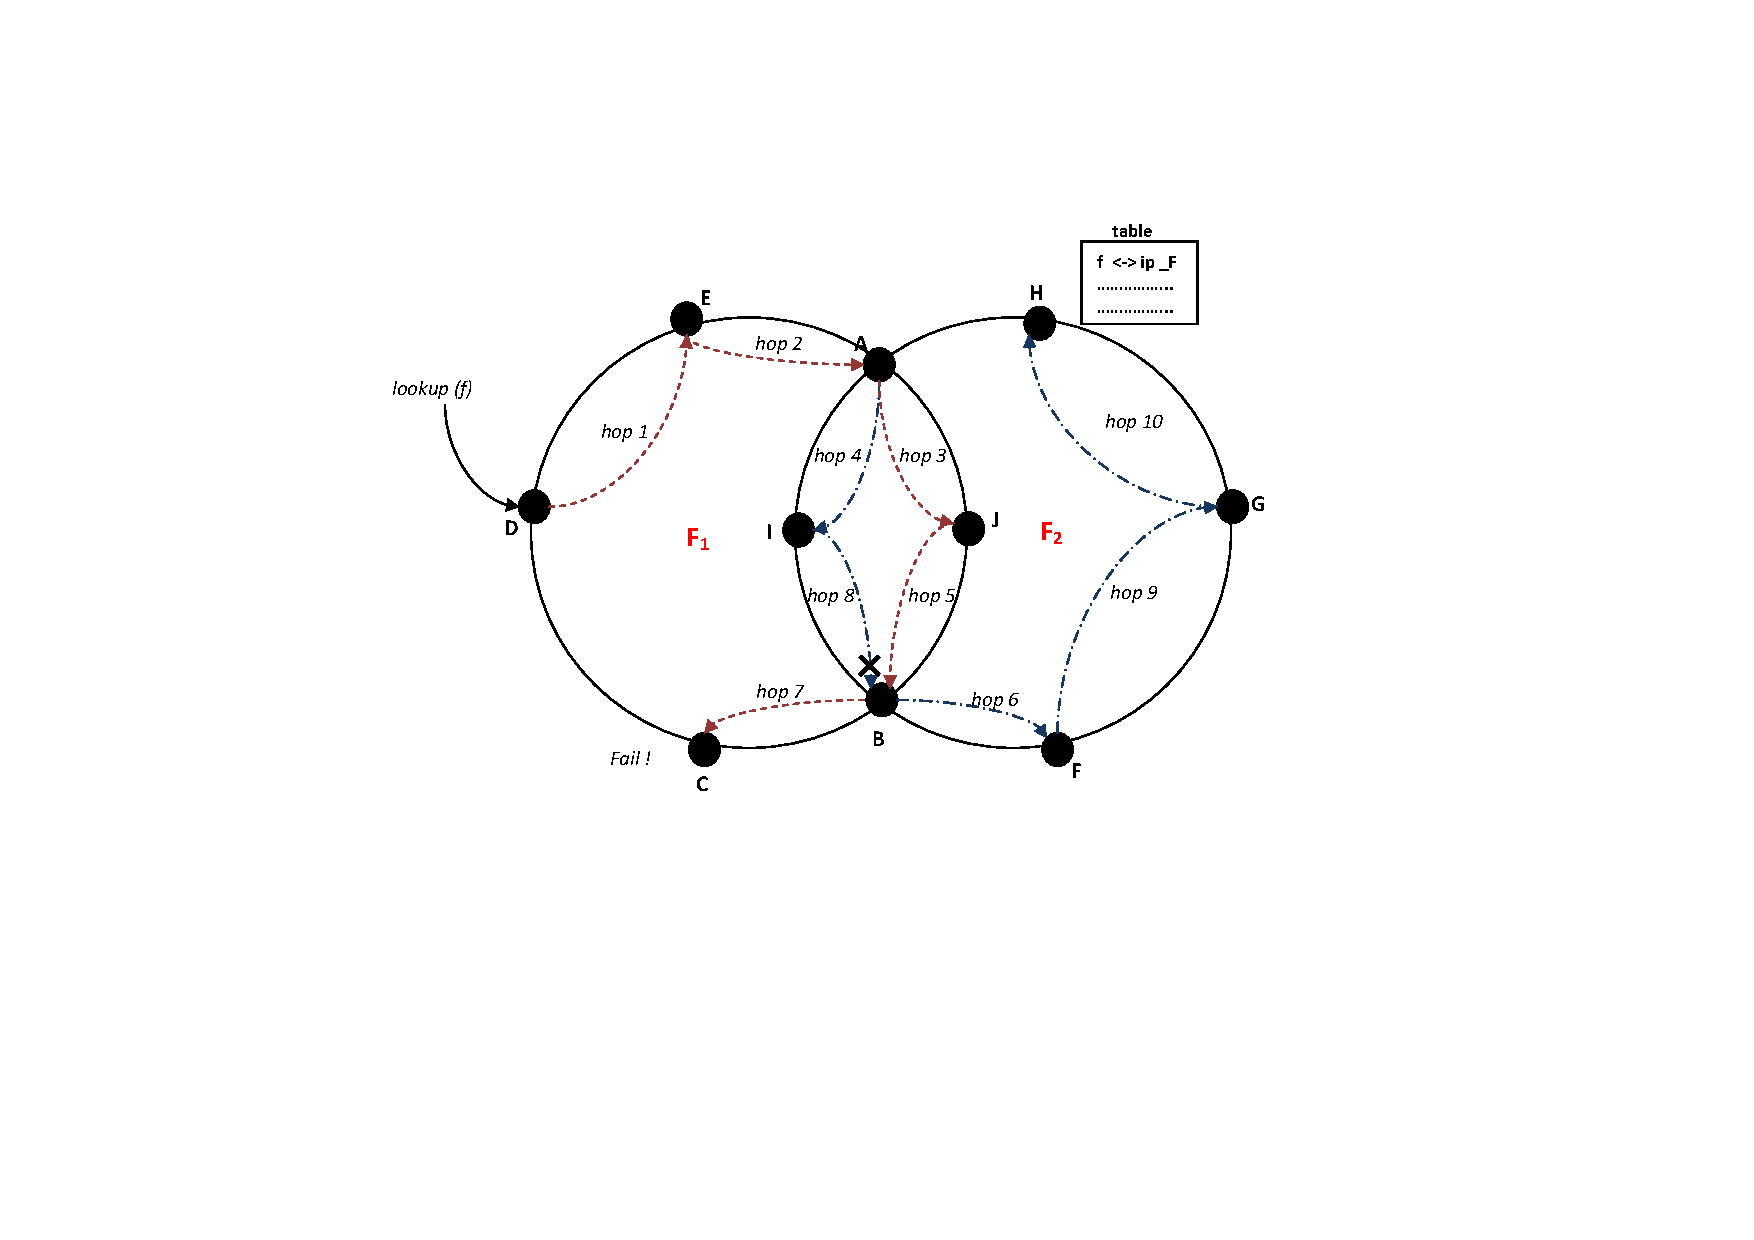
\includegraphics[width=1\linewidth]{fig/figure_example.pdf} \up{4}
  \end{center}
  \up{5}\caption{Multi-floor routing example \label{fig:multiFloorExample}}
\end{figure}

\subsection{An example}
%
We illustrate the Babelchord protocol by giving an example of a simple
two floors overlay topology and multi-floor lookup routing.
Figure~\ref{fig:multiFloorExample} shows a topology made of two floors
\verbi{F1} and \verbi{F2}. Peers are depicted by capital letters, \ie\
\verbi{A,B,..I}, and \verbi{J}. Assume that every peer offers a single
resource, \ie\ \verbi{a,b,...,i}, and \verbi{j}. The two Babelchord
floors intersect via two synapses peers \verbi{A} and \verbi{B}. Hops
are labeled by an integer \verbi{i} denoting a global time of arrival
on a given peer. Since intra-floor routing is performed as in Chord,
fingers and hand tables are hence omitted. For graphical purposes,
routing in the first floor moves clockwise, while in the second floor
moves anticlockwise. For clarity, we omit to hash peers and resources
via the two different hash functions. A \verbi{lookup(f)} is received
by peer \verbi{D} on floor \verbi{F1}; the intra-floor routing (hops
\verbi{1} and \verbi{2}) goes to \verbi{E} and \verbi{A} (the synapse)
that, in turn, will trigger an inter-floor routing on floor \verbi{F2}
(hop \verbi{4}). The routings proceed in parallel on both floors
passing by peers \verbi{I}, \verbi{J}, and \verbi{B} (hops
\verbi{3,4,5} and \verbi{8}, respectively). Since peer \verbi{B} is
the second synapse, when it receives the \verbi{lookup(f)} by hop
\verbi{8} on floor \verbi{F2}, it will not forward it since it already
saw the lookup triggered on \verbi{F1}. In the meantime, the two
lookups will continue their route to peers \verbi{C} (routing failure
on floor \verbi{F1}), on peers \verbi{F,G}, and finally terminate on
peer \verbi{H} hosting the value \verbi{ip\_F} offering the resource
\verbi{f}.

\begin{figure*}[!t]
{\scriptsize
\begin{alltt}
\textrm{\textbf{The Babelchord's protocol}}
\AL \textbf{on receipt of} LOOKUP(r) \textbf{from} ip \textbf{do}\alglabel{alg:lookupbegin}\hfill{\rm looking for peers hosting resource r}
\AL   t = new_tag(ip);\hfill{\rm new unique tag for this lookup}
\AL   this.insert_tag(t); \hfill{\rm insert tag into the tag list}
\AL   \textbf{send} FINDSUCC(t,\(\bot\),r,ip) \textbf{to} this.ip; \alglabel{alg:lookupend}\hfill{\rm send findsucc to itself}
\AL   \textbf{receive} FOUND(f,ip2) \textbf{from} ip3\hfill{\rm wait for the Babelchord routing}
\AL   \textbf{if} ping(ip2) \hfill{\rm test the aliveness of ip2}
\AL     this.update_hotpeers(ip2,f);\hfill{\rm update the hot peer list with ip2 at floor f}
\AL     this.update_hotfloors(f,ip2);\hfill{\rm update the hot floor list with f signaled by ip2}
\AL     \textbf{return} lookup_table(ip2,r);\hfill{\rm remote table lookup on ip2; return the list of ips offering the resource r}

\AL \textbf{on receipt of} FINDSUCC(t,f,r,ip) \textbf{from} ip2 \alglabel{alg:findsuccbegin}\hfill{\rm find the successor of ip}
\AL   \textbf{if} t = {join} \hfill{\rm join a floor}
\AL     \textbf{if} f(r)\( \in \)(f(this.ip),f(this.get_succ(f))]\hfill{\rm as in Chord}
\AL       \textbf{send} FOUND(f,this.get_succ(f)) \textbf{to} ip;\hfill{\rm found the successor of ip}
\AL     \textbf{else}
\AL       ip3 = this.closest_preceding_node(f,r); \hfill{\rm internal Chord routing}
\AL       \textbf{send} FINDSUCC(t,f,r,ip) \textbf{to} ip3;\hfill{\rm send to the next hop}
\AL   \textbf{else if} not(this.in_tag(t)) \hfill{\rm lookup not processed}
\AL     this.push_tag(t); \hfill{\rm mark as ``already processed''}
\AL     \textbf{for all} g\( \in \)this.dom_hands() \textbf{do}\hfill{\rm for all floors of current peer}
\AL       \textbf{if} g(r)\( \in \)(g(this.ip),g(this.get_succ(g))]\hfill{\rm test if arrived, as in Chord}
\AL         \textbf{send} FOUND(g,this.get_succ(g)) \textbf{to} ip;\hfill{\rm found a peer hosting an entry for r}
\AL         \textbf{exit forall};\hfill{\rm stop the routing: ``game over''}
\AL       \textbf{else}
\AL         ip4 = this.closest_preceding_node(g,r); \hfill{\rm internal Chord routing}
\AL         \textbf{send} FINDSUCC(t,g,r,ip) \textbf{to} ip4;\alglabel{alg:findsuccend}\hfill{\rm send findsucc to the next hop}

\textrm{\textbf{Auxiliary functions}}
\AL closest_preceding_node(f,r)\hfill{\rm internal function as in Chord}
\AL   \textbf{for} i = m \textbf{downto} 1 \textbf{do}\hfill{\rm for all fingers of floor f}
\AL     \textbf{if} this.lookup_hands(f)[i] \(\in\) (f(this.ip),f(r))\hfill{\rm testing the hand table as in Chord}
\AL       \textbf{return} this.lookup_hands(f)[i];\hfill{\rm return the finger of floor f}
\AL   \textbf{return} this.ip;\hfill{\rm return the current peer ip}
\end{alltt}} \up{5}
\caption{Pseudocode for multi-floor resource lookup \label{fig:lookup}}
\end{figure*}


\section{Babelchord's protocol}

We present the details of the algorithms to build Babelchord. First,
we focus on how Chord's variables are extended to support a
multi-floor architecture. Then, in Section~\ref{ssec:lookup}, we give
the Babelchord lookup. Finally, in Section~\ref{ssec:tower}, we give
an idea on how peers can negotiate joins and creation of floors.
Recall that words \emph{floor} and \emph{ring} refer to the same
object.

\subsection{Data structures for every peer}

Let \verbi{f}, \verbi{g} represent both the identifier of a floor and,
with a slight abuse of notation, the hash function \verbi{hash(f)(-)}
used at this floor. (We assume a distinct cryptographic hash function
for each floor). The \verbi{tag} structure is a list of unique
identifiers of previously seen requests. The \verbi{res} structure
represents the set of resources offered by a single peer, while the
\verbi{table} structure is the part of the hash table the peer
manages, containing the associative array of resource keys and
IP-addresses providing these resources. Every peer contributes
actively to routing through its \verbi{table} and to resource
exchange. The \verbi{succ}, \verbi{pred}, and \verbi{hands} structures
contain predecessor, successor and finger information for each floor.
Finally, \verbi{hotpeers} and \verbi{hotfloors} contain information
collected through lookups about peers for potential collaborations and
floors for potential participation. Here is the detailed list of
variables:


{\scriptsize
\begin{alltt}
\textrm{\textbf{Node's Data structures}}
f(-)      \(\stackrel{de\!f}{=}\) hash(f)(-)\textrm{with} hash:int->Sha1\hfill{\rm hash function}
tag       \(\stackrel{de\!f}{=}\) (int)\(\sp{*}\)\hfill{\rm list of unique tags identifying a Babelchord packet}
res       \(\stackrel{de\!f}{=}\) (r)\(\sp{*}\)\hfill{\rm list of resources offered by the current peer}
table     \(\stackrel{de\!f}{=}\) (r,(ip)\(\sp{*}\))\(\sp{*}\)\hfill{\rm the associative array of key, value pairs}
succ      \(\stackrel{de\!f}{=}\) (f,ip)\(\sp{*}\)\hfill{\rm associative array of successors at floor f}
pred      \(\stackrel{de\!f}{=}\) (f,ip)\(\sp{*}\)\hfill{\rm associative array of predecessors at floor f}
fingers   \(\stackrel{de\!f}{=}\) [ip] \hfill{\rm array of ip addresses}
hands     \(\stackrel{de\!f}{=}\) (f,fingers)\(\sp{*}\)\hfill{\rm associative array of fingers at floor f}
hotpeers  \(\stackrel{de\!f}{=}\) (ip,(f)\(\sp{*}\))\(\sp{\!*}\)\hfill{\rm\,associative\,array\,of\,peers\,view\,by\,some\,floors}
hotfloors \(\stackrel{de\!f}{=}\) (f,(ip)\(\sp{*}\))\(\sp{\!*}\)\hfill{\rm\,associative\,array\,of\,floors\,view\,by\,some\,peers}
\end{alltt}}


\begin{figure*}[!th]
{\scriptsize
\begin{alltt}\NA
\AL \textbf{on receipt of} JOIN(f) \textbf{from} ip\hfill{\rm current peer invited by ip to join f}
\AL   \textbf{if} this.good_deal(f,ip)\hfill{\rm the invitation is a ``good deal'' (strategy left to implementers)}
\AL     this.add_hands(f,\(\bot\));\hfill{\rm add floor f to the hands associative array}
\AL     this.add_succ(f,\(\bot\));\hfill{\rm add a successor for floor f to the successor associative array}
\AL     this.add_pred(f,\(\bot\));\hfill{\rm add a successor for floor f to the successor associative array}
\AL     \textbf{send} FINDSUCC(join,f,this.ip,this.ip) to ip;\hfill {\rm find my successor}
\AL     \textbf{receive} FOUND(f,ip2) \textbf{from} ip3;\hfill{\rm receiving the response}
\AL     this.reassign_succ(f,ip2);\hfill{\rm reassign ip3 as my successor at floor f}
\AL     \textbf{for all} r\( \in \)res \textbf{do}\hfill{\rm for all the resources offered by the current peer}
\AL       \textbf{send} FINDSUCC(join,f,r,this.ip) to ip;\hfill {\rm find the peer hosting the table entry for r}
\AL       \textbf{receive} FOUND(f,ip5) \textbf{from} ip4;\hfill{\rm waiting for response}
\AL       \textbf{if} ping(ip5) \hfill{\rm test the aliveness of ip5}
\AL         update_table(ip5,r,this.ip);\hfill{\rm the table stored on ip5 is updated with the new bind for r with this.ip}

\AL \textbf{on receipt of} JOINREQ(f) \textbf{from} ip\hfill{\rm the current peer ask to ip to join the floor f}
\AL   \textbf{if} this.good_deal(f,ip)\hfill{\rm accept ip at floor f is a ``good deal'' (strategy left to implementers)}
\AL     \textbf{send} JOIN(f) to ip;\hfill{\rm accept ip at floor f}
\end{alltt}} \up{4}
\caption{Pseudocode for join and join request \label{fig:join}}
\end{figure*}




\begin{figure*}[!th]
{\scriptsize
\begin{alltt}
\textrm{\textbf{Runned periodically, in order to make some inter-floor business}}\NA
\textrm{\textbf{Join a hot floor (increase local, i.e. peer, connectivity)}}
\AL join_new_floor()
\AL   \textbf{select} f\( \in \)(this.dom_hotfloors() \(\setminus\) this.dom_hands());\hfill{\rm select one floor to join (strategy left free)}
\AL   \textbf{select} ip\( \in \)this.select_node(f);\hfill{\rm select one peer of f to send a join request}
\AL     \textbf{send} JOINREQ(f) \textbf{to} ip;\hfill{\rm send an invitation to ip to join floor f}

\textrm{\textbf{Invite an hot peer to a randomly chosen floor (increase semilocal, i.e. floor, connectivity)}}
\AL  invite_new_node()
\AL    \textbf{select}  f\( \in \)this.dom_hands();\hfill{\rm select one floor to invite a peer (strategy left free to impl.)}
\AL    \textbf{select} ip\( \in \)this.dom_hotpeers();\hfill{\rm select one hot peer to invite (strategy left free to impl.)}
\AL    \textbf{if} this.good_deal(f,ip)\hfill{\rm the invitation is a ``good deal'' (strategy left to implementers)}
\AL      \textbf{send} JOIN(f) \textbf{to} ip;\hfill{\rm send an invitation to ip to join floor f}

\textrm{\textbf{Create a new floor from scratch (increase global, i.e. Babelchord, connectivity)}}
\AL  create_new_floor()
\AL    f = new_floor(ip) ;\hfill{\rm a new floor function is created}
\AL    this.add_hands(f,\(\bot\));\hfill{\rm \(\bot\) is the new floor}
\AL    this.add_pred(f,\(\bot\));\hfill{\rm \(\bot\) is the predecessor}
\AL    this.add_succ(f,ip);\hfill{\rm ip itself is the successor}
\end{alltt}} \up{6}
  \caption{Pseudocode for negotiating new joins\label{fig:business}}
\end{figure*}


\subsection{The lookup protocol \label{ssec:lookup}}
%
The multi-floor lookup is illustrated in Figure~\ref{fig:lookup}.
Lines $1.01$ to $1.04$ initiate a \verbi{lookup} on a resource
\verbi{r}. After creating a new unique tag for this request, the
current peer initiates the lookup by sending a \verbi{FINDSUCC}
message to itself, and waits for the response, \ie, a \verbi{FOUND}
message specifying the IP-address of a peer storing the sought key. On
receipt of a \verbi{FINDSUCC} message (Line $1.10$), the current peer
distinguishes two types of messages:
%
\paragraph*{Join routing (Lines 1.12-1.16).} When the first element of
the message is a \verbi{join} tag, it
means %, as we will detail later,
that the lookup serves a join purpose. The request is then routed as
in % a simple
Chord's \verbi{join}, and corresponds to the routing process of either
a resource registration or a peer insertion.
% Note that when the requested \verbi{id} falls between the current node and its successor \verbi{succ}, the node targeted by the routing is \verbi{succ}.
A \verbi{FOUND} message is then returned to the initiator of the
routing \verbi{ip} at Line $1.13$.
%
\paragraph*{Resource lookup routing (Lines 1.18-1.25).} If the first
element of the message is a numeric tag, it means that the message is
part of a resource lookup request. The message can then be routed in
several rings the current peer belongs to. First, the tag of the
request is checked (Lines $1.17$-$1.18$). If the request was already
processed, it is simply
ignored, % implementing the \emph{cut-over} strategy.
otherwise, the request tag is saved.
% in order to avoid routing the same request several times.  Note that, the requests are routed according to every floor a node belongs to.  It may be envisioned that the request may be routed to only a subset of floors, dynamically chosen by the current node, according to a local policy.  When the routing reaches its destination on a given floor, a \verbi{FOUND} message containing the address of the node storing the information of the requested resource, is sent back to the initiator of the lookup.
When a search is successful, a \verbi{FOUND} message (containing the
address of the peer responsible for the requested information) is sent
back to the lookup's initiator. On receipt of \verbi{FOUND} (Lines
$1.05$-$1.09$), the initiator checks the aliveness of the
peer % \verbi{ip} returned
and % rewards it locally by updating the reputation of \verbi{ip} in its hot
updates its hot peer and hot floor lists according to its
satisfaction. Finally, it remotely reads the values wanted (Line
$1.09$). Lines $1.26$-$1.30$ detail one local routing step (finding
the closest preceding peer among my fingers) for the next step, as in
Chord, but it includes the floor information.
% This part is very similar to the Chord local routing step, but integrating the floor information.


\subsection{New floor creation (tower building) \label{ssec:tower}}\up{2}
%
Figures~\ref{fig:join} and~\ref{fig:business} show the creation of new
floors:
% We first give the details of the receipt of two building block
% messages serving the creation of new floors:
\verbi{JOIN} and \verbi{JOINREQ}. Lines $2.01$ to $2.13$ detail the
reception of a \verbi{JOIN(f)} message which is an invitation to join
floor \verbi{f} from a peer \verbi{ip}, already member of \verbi{f}.
On receipt, the peer decides whether it is a \emph{good
  deal} or not to join \verbi{f} %according to some local information
(Line $2.02$). If this is the case, the current peer initiates its
join to \verbi{f} by sending a \verbi{FINDSUCC} message to \verbi{ip}
and waits for its information required to belong to \verbi{f}, namely,
its \verbi{successor}. On receipt, the current peer registers its
resources \verbi{res} into the floor %, one by one
(Lines $2.09$-$2.13$). Lines $2.14$ to $2.16$ detail the receipt of
the \verbi{JOINREQ(f)} message, used to request an invitation. On
receipt, the peer evaluates the advantages and drawbacks of accepting
a new peer at floor \verbi{f} and sends an invitation in the case of a
positive evaluation.

Through Figure~\ref{fig:business}, we show the pseudocode for
proposing, negotiating, and accepting new
connections. % in Babelchord.
The following functions are periodically triggered:
\verbi{join\_new\_floor} (Lines $3.01$ to $3.04$) selects one floor
(among the hot floors list) and requests an invitation to one peer of
this floor. \verbi{invite\_new\_node} (Lines $3.05$ to $3.09$) selects
a peer to invite at a given floor (this peer must reach the
\verbi{good\_deal} requirements). \verbi{create\_new\_floor} (Lines
$3.10$ to $3.14$) initiate the creation of a new floor for future
invitations.

% Note that any strategy for choosing nodes and floors can be
% implemented. Strategies may include evaluating nodes and floors
% according to performance, resources provided, presence rate, etc.

Note that the strategy for peers and floors selection can be based on
any criteria (performance, churn rate, resources' relevance\ldots).

\section{Simulation results}
%
To better capture its relevance, we have conducted some simulations of
the Babelchord approach. The simulator, written in Python, works in
two phases. First, a Babelchord topology is created, with the
following properties: (i) a fixed network size (the number of peers)
$N$, (ii) a fixed number of floors denoted $F$, (iii) a fixed global
\emph{connectivity}, \ie, the number of floors each peer belongs to,
denoted by $C$. As a consequence: (i) the peers are uniformly
dispatched among the floors, \ie, each peer belongs to $C$ floors
uniformly chosen among the set of floors, (ii) each resource provided
by peers is present at $C$ floors, (iii) the average lookup length
within one given floor is $\log((N \times C)/F)/2$.

In a second time, the simulator computes the number of hops required
to reach one of the peer storing the key of a particular resource.
Results are given for different values of $N$, $F$, and $C$.
Figure~\ref{fig:simu1} gives the results for $C{=}2$ and
$F{=}10,50,100$. Note that, in this case, the size of the routing
table is in $O(\log((N \times C)/ F)){<}O(\log(N))$. The curves
clearly demonstrates the logarithmic behavior of such an architecture,
even if the average number of hops remains slightly above the Chord
reference ($\log(N)/2 $). Note also that, the curves suggest that when
the ratio $C/F$ decreases, the lookup length increases. This statement
is rather intuitive: at each multi-floor routing step, the number of
floors reached by a request depends on this ratio.
Figure~\ref{fig:simu1} also presents the same experiments with
$C{=}5$. As expected, the lookup length is slightly reduced compared
to the results with $C{=}2$. Finally, Figure~\ref{fig:bab_last} shows
the number of synapses vs. the lookup success rate. Only 5\% of the
whole population is a synapse connecting 2 (resp. 3, 5, 10) floors.
However, this is enough to achieve more than 50\% (resp. 60\%, 80\%,
95\%) of exhaustive lookups in the Babelchord network.
%

\begin{figure}[!htb]
  \begin{center}
    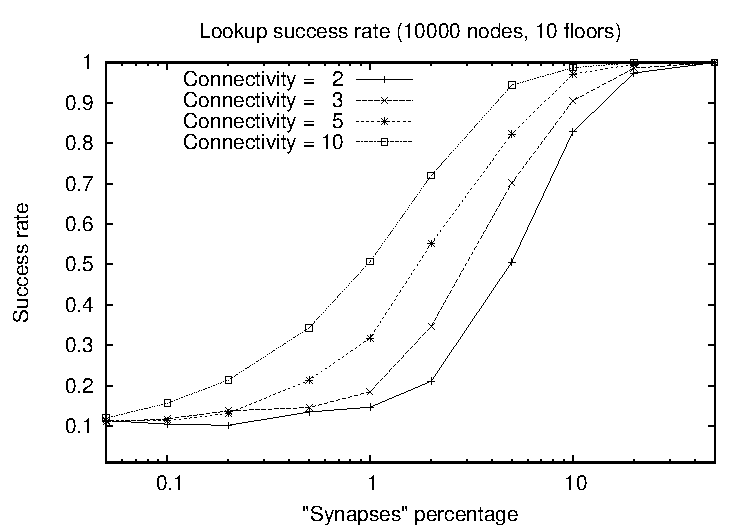
\includegraphics[width=.9\linewidth]{fig/bab_last}
    \caption{Exhaustiveness, $N{=}10000$ \label{fig:bab_last}}
  \end{center}
\end{figure}

\begin{figure}[!htb]
  \begin{center}
    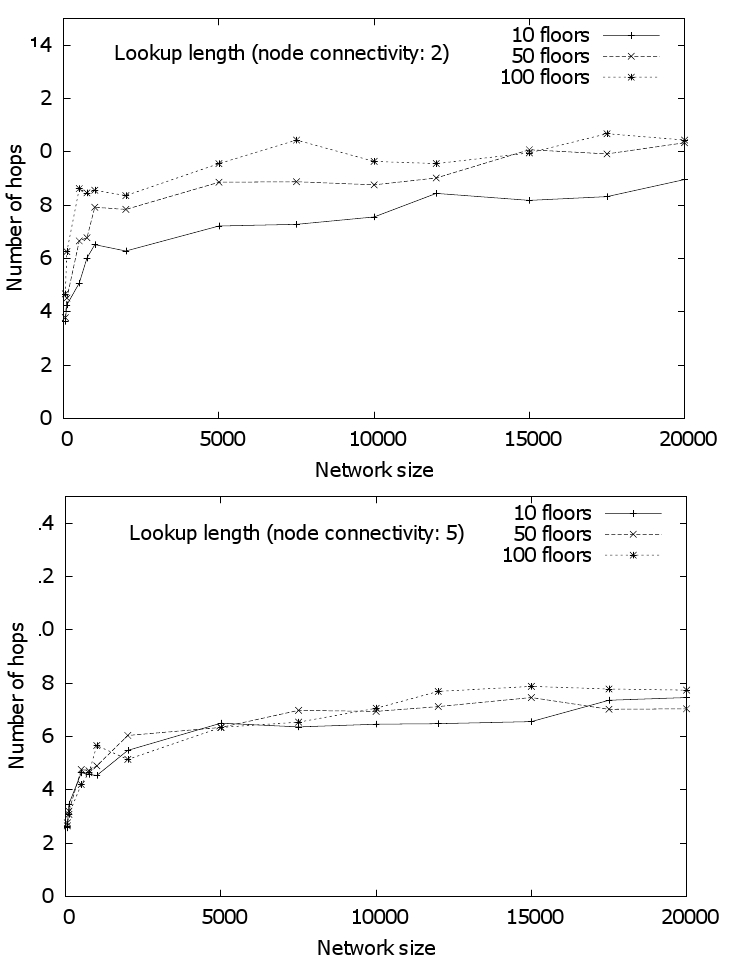
\includegraphics[width=.9\linewidth]{fig/C2andC5.jpg} \up{2}
    \caption{Lookup length, $C{=}2$ and $C{=}5$ \label{fig:simu1}}
  \end{center}
\end{figure}
%
% \begin{figure}[!htb]
%   \up{2}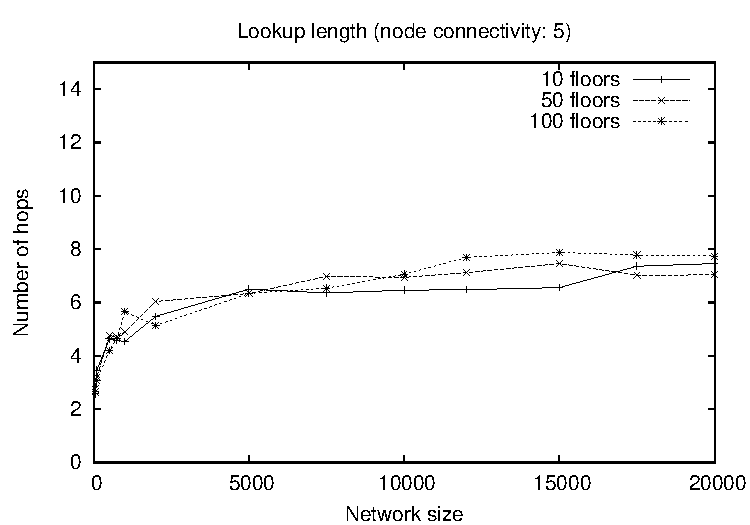
\includegraphics[width=\linewidth]{fig/bab_c5} \up{2}
%   \caption{Lookup length, $C{=}5$\label{fig:simu2}}
% \end{figure}

\up{2}
\section{Conclusion}
\up{3}
%
Babelchord is a social tower of Chord rings. It provides a simple
method to build the flexible and social next generation of overlay
networks. Babelchord aggregates smaller \emph{structured} overlay
networks in an \emph{unstructured} fashion based on intersection
peers, called \emph{synapses} allowing to explore the whole overlay
without the need for hierarchical systems or costly
merging. Simulations show that Babelchord is scalable while offering
an exhaustive search at the cost of only few synapses, thus
establishing the relevance of connecting smaller structured network in
an unstructured fashion. Next steps are a complete analysis of such
topologies, more simulations, and an actual implementation followed by
real deployments of this promising paradigm.

{\small \begin{thebibliography}{10}

  \bibitem{CCL08} R.~Chand, M.~Cosnard, and L.~Liquori. \newblock
    {Powerful Resource Discovery for Arigatoni Overlay Network}.
    \newblock {\em Future Generation Computer Systems}, 1(21):31--38,
    2008.

  \bibitem{Datta} A.~Datta and K.~Aberer. \newblock The Challenges of
    Merging Two Similar Structured Overlays: {A} tale of Two Networks.
    \newblock In {\em Proc. of IWSOS}, 2006.

  \bibitem{Biersack} L.~Erice, E.~Biersack, K.~Ross, P.~Felber, and
    G.~Keller. \newblock Hierarchical P2P Systems. \newblock In {\em
      Euro-Par}, 2003.

  \bibitem{Biersack2} L.~Erice, K.~Ross, E.~Biersack, P.~Felber, and
    G.~Keller. \newblock Topology-Centric Look-up Service. \newblock
    In {\em NGC}, 2003.

  \bibitem{LC07b} L.~Liquori and M.~Cosnard. \newblock {Logical
      Networks: Towards Foundations for Programmable Overlay
      Networks and Overlay Computing Systems}. \newblock In {\em TGC},
    volume 4912 of {\em LNCS}, pages 90--107. Springer,
    2007.

  \bibitem{CAN} S.~Ratnasamy, P.~Francis, M.~Handley, R.~Karp, and
    S.~Shenker. \newblock {A Scalable Content-Adressable Network}.
    \newblock In {\em ACM SIGCOMM}, 2001.

  \bibitem{Haridi} T.~Shafaat, A.~Ghodsi, and S.~Haridi. \newblock
    Handling Network Partitions and Mergers in Structured Overlay
    Networks. \newblock In {\em Proc. of P2P}, pages 132--139. IEEE
    Computer Society, 2007.

  \bibitem{Chord} I.~Stoica, R.~Morris, D.~Karger, M.~Kaashoek, and
    H.~Balakrishnan. \newblock {Chord: A Scalable Peer-to-Peer Lookup
      service for Internet
      Applications.} \newblock In {\em ACM SIGCOMM}, pages 149--160,
    2001.

  \bibitem{brocade} B.~Zhao, Y.~Duan, L.~Huang, A.~Joseph, and
    J.~Kubiatowicz. \newblock {Brocade: Landmark Routing on Overlay
      Networks}. \newblock In {\em IPTPS}, 2002.

  \end{thebibliography}
}
\end{document}
